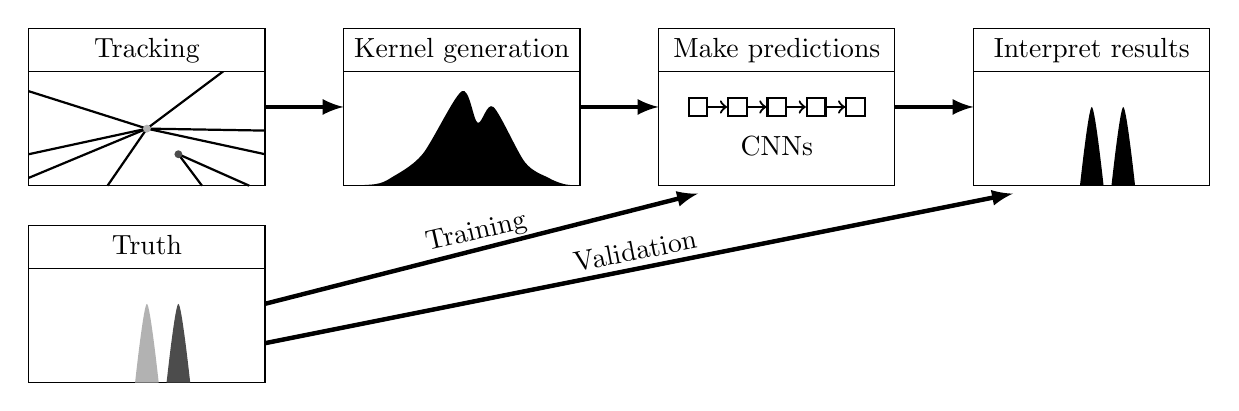
\begin{tikzpicture}[
    scale=1,
    belowbox/.style={draw},
    topbox/.style={draw, fill=white},
    texttop/.style={below},
    track/.style={thick},
    minibox/.style={draw, thick, minimum width=.1cm, minimum height=.1cm},
    miniarr/.style={->, thick},
    conn/.style={-latex, ultra thick}
    ]
    	\begin{scope}
    	    \path [belowbox] (-1.5,-1) rectangle (1.5,.45);
    		\draw [track] (0,-.275) -- (-1.5,-.9);
    		\draw [track] (0,-.275) -- (-1.5,-.6);
    		\draw [track] (0,-.275) -- (-1.5,.2);
    		\draw [track] (0,-.275) -- (1.5,-.3);
    		\draw [track] (0,-.275) -- (1.5,-.6);
    		\draw [track] (0,-.275) -- (1.5,.85);
    		\draw [track] (0,-.275) -- (-.5,-1);
    		\draw [track] (.4, -.6) -- (1.3,-1);
    		\draw [track] (.4, -.6) -- (.7,-1);
    		\path [topbox]  (-1.5,.45) rectangle (1.5,1);
    	    \node at (0,1) [texttop] {Tracking};
            \path [fill=black!30] (0, -.275) circle (.05);
            \path [fill=black!70] (.4, -.6) circle (.05);
    	\end{scope}

    	\begin{scope}[xshift=4cm]
    	    \path [belowbox] (-1.5,-1) rectangle (1.5,.45);
    		\path [fill=black] plot [smooth] coordinates {
    			(-1.5,-1)
    			(-1.1, -.98)
    			(-.9, -.9)
    			(-.5, -.6)
    			(0, .2)
    			(.2, -.2)
    			(.4, 0)
    			(.8, -.7)
    			(1.1, -.9)
    			(1.3, -.98)
    			(1.5,-1)
    		};
    		\path [topbox]  (-1.5,.45) rectangle (1.5,1);
    	    \node at (0,1) [texttop] {Kernel generation};
    	\end{scope}

    	\begin{scope}[xshift=8cm]
    	    \path [belowbox] (-1.5,-1) rectangle (1.5,.45);

            \begin{scope}[yshift=3mm]
        		\node [minibox] (mA) at (-1,-.3) {};
        		\node [minibox] (mB) at (-.5,-.3) {};
        		\node [minibox] (mC) at (0,-.3) {};
        		\node [minibox] (mD) at (.5,-.3) {};
        		\node [minibox] (mE) at (1,-.3) {};
        		\draw [miniarr] (mA) -- (mB);
        		\draw [miniarr] (mB) -- (mC);
        		\draw [miniarr] (mC) -- (mD);
        		\draw [miniarr] (mD) -- (mE);
            \end{scope}

    		\path [topbox]  (-1.5,.45) rectangle (1.5,1);
    	    \node at (0,1) [texttop] {Make predictions};
            \node at (0,-.5) {CNNs};
    	\end{scope}

    	\begin{scope}[xshift=12cm]
    	    \path [belowbox] (-1.5,-1) rectangle (1.5,.45);
    		\path [fill=black] plot [smooth] coordinates {
    		(-.15,-1)
    		(0, 0)
    		(.15,-1)
    		};
    		\path [fill=black] plot [smooth] coordinates {
    		(.25,-1)
    		(.4, 0)
    		(.55,-1)
    		};
    		\path [topbox]  (-1.5,.45) rectangle (1.5,1);
    	    \node at (0,1) [texttop] {Interpret results};
    	\end{scope}

    	\begin{scope}[xshift=0cm, yshift=-2.5cm]
    	    \path [belowbox] (-1.5,-1) rectangle (1.5,.45);
    		\path [fill=black!30] plot [smooth] coordinates {
    		(-.15,-1)
    		(0, 0)
    		(.15,-1)
    		};
    		\path [fill=black!70] plot [smooth] coordinates {
    		(.25,-1)
    		(.4, 0)
    		(.55,-1)
    		};
    		\path [topbox]  (-1.5,.45) rectangle (1.5,1);
    	    \node at (0,1) [texttop] {Truth};
    	\end{scope}

    	\draw [conn] (1.5,0) -- (2.5,0);
    	\draw [conn] (5.5,0) -- (6.5,0);
    	\draw [conn] (9.5,0) -- (10.5,0);
    	\draw [conn] (1.5, -2.5) -- (7, -1.1) node [above=-2.5, midway, rotate=13] {Training};
    	\draw [conn] (1.5, -3) -- (11, -1.1) node [above=-1, midway, rotate=11] {Validation};
\end{tikzpicture}